%
% This is the LaTeX template file for lecture notes for EE 382C/EE 361C.
%
% To familiarize yourself with this template, the body contains
% some examples of its use.  Look them over.  Then you can
% run LaTeX on this file.  After you have LaTeXed this file then
% you can look over the result either by printing it out with
% dvips or using xdvi.
%
% This template is based on the template for Prof. Sinclair's CS 270.

\documentclass[twoside]{article}
\usepackage{graphicx}
\usepackage{wrapfig}
\usepackage{amsmath}
\usepackage{amssymb}
\usepackage{listings}
\setlength{\oddsidemargin}{0.25 in}
\setlength{\evensidemargin}{-0.25 in}
\setlength{\topmargin}{-0.6 in}
\setlength{\textwidth}{6.5 in}
\setlength{\textheight}{8.5 in}
\setlength{\headsep}{0.75 in}
\setlength{\parindent}{0 in}
\setlength{\parskip}{0.1 in}

%
% The following commands set up the lecnum (lecture number)
% counter and make various numbering schemes work relative
% to the lecture number.
%
\newcounter{lecnum}
\renewcommand{\thepage}{\thelecnum-\arabic{page}}
\renewcommand{\thesection}{\thelecnum.\arabic{section}}
\renewcommand{\theequation}{\thelecnum.\arabic{equation}}
\renewcommand{\thefigure}{\thelecnum.\arabic{figure}}
\renewcommand{\thetable}{\thelecnum.\arabic{table}}

%
% The following macro is used to generate the header.
%
\lstset{language=Python, numbers=left, tabsize=2, xleftmargin=5.0ex}

\newcommand{\lecture}[4]{
   \pagestyle{myheadings}
   \thispagestyle{plain}
   \newpage
   \setcounter{lecnum}{#1}
   \setcounter{page}{1}
   \noindent
   \begin{center}
   \framebox{
      \vbox{\vspace{2mm}
    \hbox to 6.28in { {\bf EE 382N: Distributed Systems
                        \hfill Fall 2017} }
       \vspace{4mm}
       \hbox to 6.28in { {\Large \hfill Lecture #1: #2  \hfill} }
       \vspace{2mm}
       \hbox to 6.28in { {\it Lecturer: #3 \hfill Scribe: #4} }
      \vspace{2mm}}
   }
   \end{center}
   \markboth{Lecture #1: #2}{Lecture #1: #2}
   %{\bf Disclaimer}: {\it These notes have not been subjected to the
   %usual scrutiny reserved for formal publications.  They may be distributed
   %outside this class only with the permission of the Instructor.}
   \vspace*{4mm}
}

%
% Convention for citations is authors' initials followed by the year.
% For example, to cite a paper by Leighton and Maggs you would type
% \cite{LM89}, and to cite a paper by Strassen you would type \cite{S69}.
% (To avoid bibliography problems, for now we redefine the \cite command.)
% Also commands that create a suitable format for the reference list.
\renewcommand{\cite}[1]{[#1]}
\def\beginrefs{\begin{list}%
        {[\arabic{equation}]}{\usecounter{equation}
         \setlength{\leftmargin}{2.0truecm}\setlength{\labelsep}{0.4truecm}%
         \setlength{\labelwidth}{1.6truecm}}}
\def\endrefs{\end{list}}
\def\bibentry#1{\item[\hbox{[#1]}]}

%Use this command for a figure; it puts a figure in wherever you want it.
%usage: \fig{NUMBER}{SPACE-IN-INCHES}{CAPTION}
\newcommand{\fig}[3]{
			\vspace{#2}
			\begin{center}
			Figure \thelecnum.#1:~#3
			\end{center}
	}
% Use these for theorems, lemmas, proofs, etc.
\newtheorem{theorem}{Theorem}[lecnum]
\newtheorem{lemma}[theorem]{Lemma}
\newtheorem{proposition}[theorem]{Proposition}
\newtheorem{claim}[theorem]{Claim}
\newtheorem{corollary}[theorem]{Corollary}
\newtheorem{definition}[theorem]{Definition}
\newenvironment{proof}{{\bf Proof:}}{\hfill\rule{2mm}{2mm}}

% **** IF YOU WANT TO DEFINE ADDITIONAL MACROS FOR YOURSELF, PUT THEM HERE:

\begin{document}
%FILL IN THE RIGHT INFO.
%\lecture{**LECTURE-NUMBER**}{**DATE**}{**LECTURER**}{**SCRIBE**}
\lecture{1}{Aug 18}{Vijay Garg}{Pankaja A}
%\footnotetext{These notes are partially based on those of Nigel Mansell.}

% **** YOUR NOTES GO HERE:

% Some general latex examples and examples making use of the
% macros follow.  
%**** IN GENERAL, BE BRIEF. LONG SCRIBE NOTES, NO MATTER HOW WELL WRITTEN,
%**** ARE NEVER READ BY ANYBODY.
\section{Introduction}
This is the first lecture for this course. The professor started with a walk-through of course contents and grading policy.Please refer to canvas for this information.

The main topics discussed in this lecture are:

\begin{itemize}
	\item Goals of the course
	\item What are distributed systems
	\item Puzzles
\end{itemize}

This set of lecture notes will briefly re-examine the topics covered in this lecture, in the order in which they appeared during class. 

\section{Goals of the course}

The goals of this course is to have basic understanding of the topics listed in syllabus(refer canvas). At the end of this course, write programs using sockets.

\section{What are distributed systems?}

\subsection{Concepts: Time}
Consider two events $e$ and $f$ in sequential world. Lets say event $e$ happened at $08:50$ and event $f$ happened at $08:55$.  Now, just based on the time at which these two events happened, we can certainly say that "$f$ must have happened after $e$". This only holds good for sequential world though.


Now lets consider distributed world. In distributed systems, it is impossible to synchronize the clocks. The only way to synchronize is to send messages and receive messages.

Say we have a process $P1$ running. In sequential world it is possible to get one particular instance of this execution and obtain its value. This is possible as there is a shared memory and also the clocks are synchronized.


But, in distributed systems - there is no shared clock and there are no synchronized clocks.Hence it is not possible to define one particular instance in the execution of all these processes. Also, remember that these process are running at different locations, one process may be running in one room and other process may be running in some remote satellite.

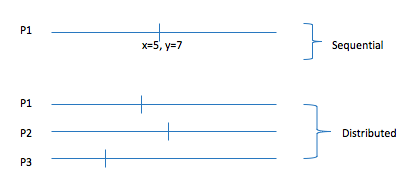
\includegraphics[scale=0.7]{images/Global_state.png}

\subsection{Centralized v/s Distributed}

Consider the centralized system as pictured below.

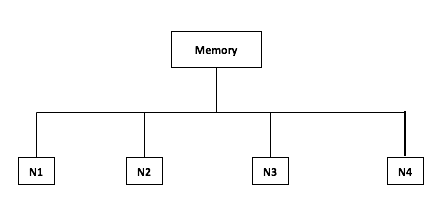
\includegraphics[scale=0.7]{images/centralized.png}

N1,N2,N3,N4 are the nodes and the memory is shared by all the nodes. Memory is not scale-able here and thus it is bottleneck.

In Distributed system( as pictured below], all the nodes are connected via a communication network.Every node has its own memory, and there  is no shared memory.

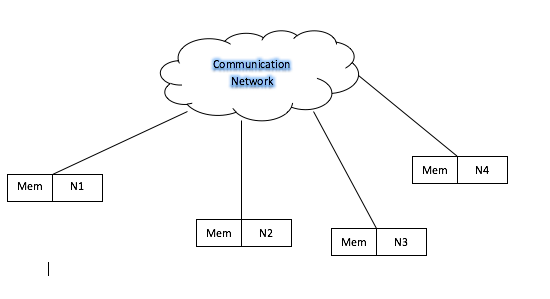
\includegraphics[scale=0.7]{images/distributed.png}

Lets say, if a node $N1$ sends message to another node $N2$. If $N1$ does not hear back from $N2$ - there can be two possibilities. Either node $N2$ is dead or the communication link itself is slow. Since its not possible to differentiate between these two cases, agreeing on a particular state would be a problem.

Thus a Distributed system is the one which has
\begin{itemize}
   \item No shared memory
   \item No shared clock
   \item No perfect failure detection
\end{itemize}




\section{Puzzles}
We covered two puzzles in this lecture.
\subsection{Byzantine general agreement problem}

This problem was introduced by 3 people - Lamport, Shostak and Pease in 1982.

This problem is built around an imaginary General who makes a decision to attack or retreat, and must communicate the decision to his lieutenants/other generals so that the resulting action is coordinated - either all attack or all retreat.

Some of these generals are disloyal.

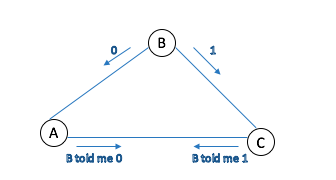
\includegraphics[scale=0.7]{images/ABC.png}

Consider a system of 3 generals, and lets say one of them (B) is disloyal.
B sends message 0(retreat) to A and sends message 1( attack) to C. Now A and C try to validate their messages, nothing can be inferred as to who is disloyal and sending conflicting messages. Its equally possible that A or C is disloyal and sending wrong message even when B send them consistent message.

Thus when the number of nodes is 3, and if there is 1 disloyal general, there is no solution.

To generalize,if $1/3$$^r^d$ of the people are disloyal then there is no solution.

\subsection{Alice,Eve and Bob}


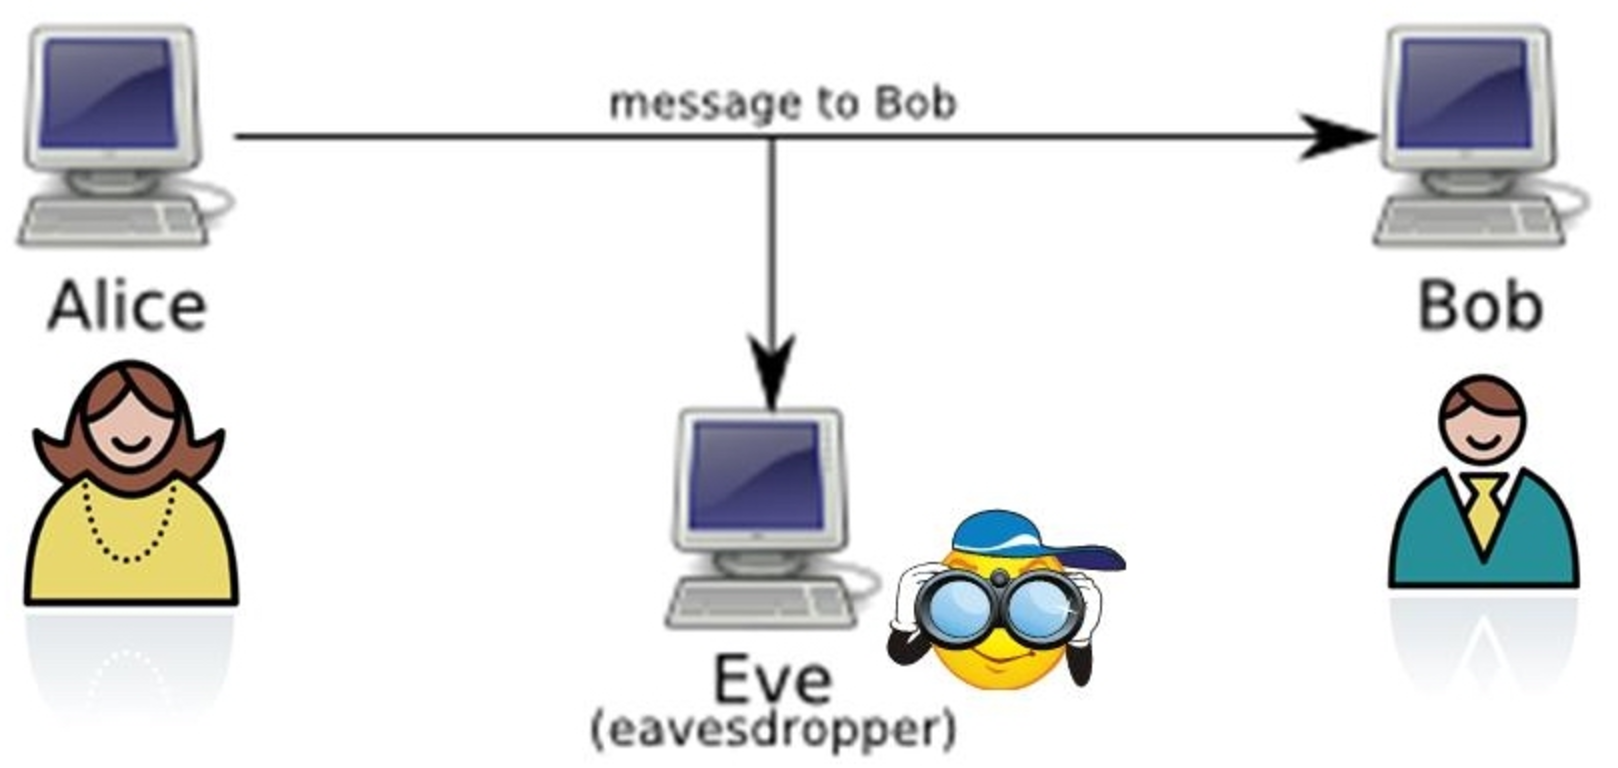
\includegraphics[scale=0.7]{images/Alice.png}

This puzzle has 3 people - Alice, Eve and Bob. Alice is calling Bob for the first time to arrange for a movie/dinner date. Now, there is Eve who is listening to the conversion( on a line) between Alice and Eve. There is nothing shared between Alice and Bob.The goal is Alice needs to communicate the intended place/time for a date to Bob without Eve getting any information regarding the same.

Solution 1:
\begin{itemize}
   
\item
Alice prepares her message, put a lock on the message and sends to Bob.
\item
Bob receives the message, puts his lock on the same message and sends back to Alice.
\item
Alice receives the message from Bob, Alice removes her lock and sends the message back to Bob, He removes his lock and he can read the message.
\end{itemize}

The assumption for this solution to work is that the encryption is commutative.


Solution 2:

\begin{itemize}
\item
Bob sends his public key to Alice
\item
Alice encrypts it and send it back to Bob. Bob can then decrypt it and read the message
\end{itemize}

\section{$P$ v/s $NP$}

There was a question asked by one student regarding $P$ v/s $NP$ problems, so professor briefly covered it in response to his question.

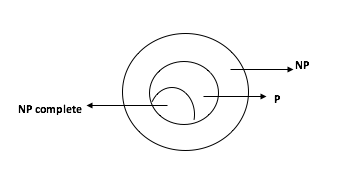
\includegraphics[scale=0.7]{images/NP.png}

Most people believe $P$$\neq$$NP$

$NP$ problems is a class of problems using which one can verify efficiency.

$P$ problems is a class of problems using which one can compute solutions efficiently.


Both $P$ and $NP$ problems will be covered in detail in subsequent lectures.

\end{document}